\documentclass[12pt, a4paper]{article}
\usepackage{graphicx}
\usepackage{amsmath}
\usepackage{algorithm}
\usepackage{algpseudocode}
\usepackage{makecell}
\usepackage{longtable}
\usepackage{float}
\usepackage{placeins}
\usepackage[utf8]{inputenc}
\usepackage[T5]{fontenc}
\usepackage[vietnamese, main=english]{babel}
\usepackage{tabularx}
\usepackage{array}
\usepackage{ragged2e}
\usepackage{setspace}
\usepackage{titlesec}
\usepackage{enumitem}
\usepackage{caption}
\usepackage[none]{hyphenat}
\captionsetup[figure]{font=small,labelfont=bf}
\captionsetup[algorithm]{font=small,labelfont=bf}
\usepackage{fancyhdr}
\usepackage{hyperref}
\fancyhf{} % Xóa hết các cài đặt header/footer mặc định

\setlength{\headheight}{26pt} % Tăng độ cao header để chứa được 2 dòng
\addtolength{\topmargin}{-14pt} % Bù lại khoảng cách lề trên
% Cấu hình Header
\lhead{Project 2} % Bên trái: Report Title
\rhead{UNIVERSITY OF SCIENCE, VNU-HCM\\
CSC14003} % Bên phải: Trường + Môn học
% Cấu hình Footer (ví dụ số trang ở giữa)
\cfoot{\thepage}
% Độ dày đường kẻ ngang ở header và footer
\renewcommand{\headrulewidth}{0.4pt}
\renewcommand{\footrulewidth}{0pt}

\setstretch{1.15}
\setlist{nosep}
\titleformat{\section}{\large\bfseries}{\thesection.}{0.5em}{}
\titleformat{\subsection}{\normalsize\bfseries}{\thesubsection.}{0.5em}{}
\hyphenpenalty=10000
\exhyphenpenalty=10000
\emergencystretch=2em

\begin{document}
\pagestyle{empty}
\begin{titlepage}
\centering

% Logo - Điều chỉnh scale nếu cần để tiết kiệm diện tích

\includegraphics[scale=0.4]{image/hcmus-logo.png}\\[0.5cm]

\textsc{\Large University of Science - VNU HCM}\\[0.2cm]
\textsc{\Large Faculty of Information Technology}\\[1.5cm]

% Tiêu đề đồ án
{\Huge \textbf{Project Report}}\\[1.5cm]

% Phần thông tin Project - Sử dụng bảng để format thẳng hàng và đẹp hơn
\begin{minipage}{0.8\textwidth}
    \large
    \textbf{Project Title:} \textit{ Freecell Solver} \\[0.5cm]
    \textbf{Course:} \textit{Introduction to Artificial Intelligence} \\[0.5cm]
    \textbf{Instructor:} \textit{Nguyễn Thanh Tình}
\end{minipage}

\vspace{1.5cm}


\newline

\vfill % Tự động đẩy phần ngày tháng xuống sát đáy trang

% Thông tin nộp bài
{\large Semester: \textit{II (2025 - 2026)}}

\end{titlepage}
\clearpage

\pagenumbering{roman}
\tableofcontents
\newpage
\listoftables
\newpage
\listoffigures
\clearpage
\pagenumbering{arabic}
\setcounter{page}{1}
\pagestyle{fancy}

\section{Introduction}
\subsection{Project Overview}
This project builds a full pipeline for solving \textit{Futoshiki} puzzles in CSC14003 --- Introduction to Artificial Intelligence. A Futoshiki puzzle is an \(N \times N\) grid where each row/column must contain \(1..N\) exactly once and all adjacency inequalities must hold.

The system is modular: I/O, domain model, knowledge base, solver modules, and GUI. It supports loading multiple inputs, running selected methods, and exporting standardized outputs. This report presents all five implemented solver families: Forward Chaining, Backward Chaining, A* Search, Brute-force/Backtracking, and SAT solving. The PySAT-based solver acts as a reliable validator to confirm the logical integrity of our core algorithms and test instances.

\subsection{Objectives and Scope}
The main objectives of this project are:
\begin{itemize}
	\item Model Futoshiki constraints consistently for search-based and logic-based solving.
	\item Implement and evaluate AI solvers with modular, reusable code.
	\item Provide a practical GUI for puzzles of different sizes.
	\item Compare methods by correctness and efficiency.
\end{itemize}

Scope of this report:
\begin{itemize}
	\item Present the overall project context.
	\item Describe all implemented solvers in detail: \textbf{Forward Chaining}, \textbf{Backward Chaining}, \textbf{A* Search}, \textbf{Brute-force/Backtracking}, and \textbf{SAT Solver (using a SAT library)}.
	\item Compare these methods through a unified experiment and GUI workflow.
\end{itemize}

\subsection{Team Information}
The project was completed by four students from the Faculty of Information Technology, University of Science --- VNU-HCM:
\begin{itemize}
	\item Nguyễn Khánh Toàn --- MSSV: 24127252
	\item Nguyễn Chí Tài --- MSSV: 24127529
	\item Nguyễn Ngọc Thiên --- MSSV: 24127545
	\item Phan Quang Tiến --- MSSV: 24127250
\end{itemize}

The team collaborated on modeling, implementation, testing, and reporting; detailed assignments are listed in the planning section.

\section{Project Planning and Task Distribution}

To ensure the project's progress and transparency, our team utilized Jira for task management and workload distribution. The project was divided into three main phases: Phase 1 (Foundation), Phase 2 (Algorithm Implementation), and Phase 3 (Evaluation and Reporting).

\subsection{Detailed Task Assignment}
Below is the summary of responsibilities and contribution for each member:

\begin{table}[!ht] % Thay [H] bằng [!ht] để LaTeX linh hoạt hơn
    \centering
    \small % Thu nhỏ chữ một chút để bảng gọn hơn, tránh nhảy trang
    \renewcommand{\arraystretch}{1.2} % Giảm từ 1.4 xuống 1.2 để tiết kiệm diện tích
    
    % Định nghĩa lại cột X để căn trái, tránh lỗi gạch nối từ ngữ
    \newcolumntype{L}{>{\raggedright\arraybackslash}X} 
    
    \begin{tabularx}{\textwidth}{|l|c|L|c|}
        \hline
        \textbf{Member Name} & \textbf{Student ID} & \textbf{Key Responsibilities (Jira Tasks)} & \textbf{Contrib.} \\ \hline
        
        Phạm Trần Anh Quân & 24127226 & 
        $\bullet$ GUI Framework \newline 
        $\bullet$ DFS Algorithm \newline 
        $\bullet$ Data Visualization & 100\% \\ \hline
        
        Nguyễn Khánh Toàn & 24127252 & 
        $\bullet$ GUI Controls \& Utilities \newline 
        $\bullet$ UCS Algorithm \newline 
        $\bullet$ Demo Video Production & 100\% \\ \hline
        
        Hồ Đình Trí & 24127254 & 
        $\bullet$ State Design \& Initialization \newline 
        $\bullet$ A* Algorithm \newline 
        $\bullet$ Algorithm Analysis \& Reporting & 100\% \\ \hline
        
        Nguyễn Tiến Cường & 24127337 & 
        $\bullet$ Actions Logic \newline 
        $\bullet$ BFS Algorithm \newline 
        $\bullet$ Experiments \& Data Collection & 100\% \\ \hline
    \end{tabularx}
    \caption{Project task distribution and member contributions.}
\end{table}

\subsection{Project Management Board}
Our team manages all issues and sprints through an online Jira board. The status of each task is tracked in real-time to ensure the project meets the deadline.

\textbf{Jira Board Link:} \href{https://dinhtri.atlassian.net/jira/software/projects/KAN/list?jql=project+%3D+KAN+ORDER+BY+created+DESC&atlOrigin=eyJpIjoiZjRkYjE0ODVkZDA4NGRjOGE5ZWE0MWFkNjM0ZGY3OTUiLCJwIjoiaiJ9}{Click here}

\textbf{Link Demo:} \href{https://youtube.com/}{Click to see video}


\section{Problem Formulation}

  FreeCell can be modeled as a deterministic, fully observable, single-agent search problem
  \[
  P = (\mathcal{S}, \mathcal{A}, T, s_0, G, c),
  \]
  where \(\mathcal{S}\) is the set of legal game states, \(\mathcal{A}\) is the set of legal actions, \(T\) is the transition model, \(s_0\) is the
  initial state, \(G\) is the goal test, and \(c\) is the step-cost function. Since all cards are visible from the beginning and no randomness appears
  after the initial deal, FreeCell is well suited for classical state-space search.

  \subsection{State Representation}

  A state \(n \in \mathcal{S}\) is represented as
  \[
  n = \bigl(\langle C_1, C_2, \dots, C_8 \rangle,\; \langle E_1, E_2, E_3, E_4 \rangle,\; \langle F_C, F_D, F_H, F_S \rangle \bigr),
  \]
  where:
  \begin{itemize}
      \item \(C_i\) is the \(i\)-th cascade (tableau column), represented as an ordered list of cards;
      \item \(E_j\) is the \(j\)-th free cell, which is either empty or contains exactly one card;
      \item \(F_s\) denotes the current top rank stored in the foundation of suit \(s \in \{C,D,H,S\}\), with \(0\) meaning that the foundation is
  empty.
  \end{itemize}

  Each card is represented by its \emph{rank} and \emph{suit}, i.e.,
  \[
  \text{card} = (r, s),
  \]
  where \(r \in \{1,\dots,13\}\) and \(s \in \{C,D,H,S\}\). In particular, \(r=1\) denotes Ace, \(r=11\) denotes Jack, \(r=12\) denotes Queen, and
  \(r=13\) denotes King.

  \subsection{Initial State}

  The initial state \(s_0\) is generated from a standard 52-card deck dealt face-up into 8 cascades. Specifically:
  \begin{itemize}
      \item 4 cascades contain 7 cards each;
      \item 4 cascades contain 6 cards each;
      \item all 4 free cells are empty;
      \item all 4 foundation piles are empty.
  \end{itemize}

  Formally, in the initial state,
  \[
  E_1 = E_2 = E_3 = E_4 = \emptyset
  \quad \text{and} \quad
  F_C = F_D = F_H = F_S = 0.
  \]

  \subsection{Actions (Transition Model)}

  From a state \(n\), a legal action corresponds to one valid move under the standard FreeCell rules. The transition model \(T(n,a)\) deterministically
  returns the unique successor state obtained after applying action \(a\).

  \begin{description}
      \item[Single-card moves.]
      A single top card from a cascade, or a card currently stored in a free cell, may be moved to:
      \begin{itemize}
          \item an empty free cell;
          \item another cascade, if it forms a descending alternating-color sequence with the destination top card;
          \item an empty cascade;
          \item its corresponding foundation, if it has the same suit and its rank is exactly one greater than the current top rank of that foundation.
      \end{itemize}

      \item[Sequence moves between cascades.]
      A sequence of cards may be moved from one cascade to another if:
      \begin{itemize}
          \item the moved sequence itself is a valid descending alternating-color sequence; 
          \item its length does not exceed the move capacity allowed by the current number of empty free cells and empty cascades.
      \end{itemize}
  \end{description}

  Let \(m\) be the number of empty free cells and let \(e\) be the number of empty cascades available as intermediate storage (excluding the
  destination cascade when it is empty). Then the maximum number of cards that can be moved together is
  \[
  ( m + 1 ) 2^e.
  \]

  Thus, a sequence move of length \(k\) is legal only if
  \[
  k \le (m+1)2^e.
  \]

  \subsection{Goal Test}

  A state \(n\) is a goal state if all cards have been moved to the foundations. Equivalently,
  \[
  G(n) = \text{true}
  \quad \Longleftrightarrow \quad
  F_C = F_D = F_H = F_S = 13.
  \]
  This is equivalent to saying that the total number of cards in the foundations is 52:
  \[
  F_C + F_D + F_H + F_S = 52.
  \]

  \subsection{Path Cost}

\subsubsection{Standard Unit-Cost Model}
In the general formulation of FreeCell, we primarily adopt a \textbf{unit-cost model}. Every legal move—including single-card moves and valid sequence moves—is assigned a cost of 1. Thus, if a path from the initial state $s_0$ to a state $n$ consists of $d$ legal moves, the path cost is defined as:
\[
g(n) = d.
\]
Equivalently, for any action $a$:
\[
c(n,a,n') = 1.
\]
Under this formulation, $g(n)$ measures the total number of moves made so far. To remain consistent with this model, any heuristic $h(n)$ used in informed search (such as $A^*$) estimates the remaining cost in the same unit: the number of moves. This model ensures that BFS, IDS, and $A^*$ find the \textbf{optimal solution} in terms of the minimum number of steps.

\subsubsection{Weighted Strategic Cost Model (UCS Implementation)}
To guide the \textbf{Uniform-Cost Search (UCS)} more efficiently through the state space, we implement a \textbf{weighted cost model} as detailed in Algorithm 7 and the source code \texttt{ucs.py}. This model assigns dynamic costs based on the strategic value of each move:

\begin{table}[h]
\centering
\begin{tabular}{|l|c|l|}
\hline
\textbf{Move Type} & \textbf{Cost} & \textbf{Strategic Reasoning} \\ \hline
To Foundation & 1 & Highest priority; directly advances toward the goal. \\ \hline
Emptying a Cascade & 5 & High priority; creates empty columns for better mobility. \\ \hline
Cascade to Cascade & 10 & Standard move; default cost for tableau maneuvers. \\ \hline
To Free Cell & 50 & Penalty cost; discourages filling limited storage slots. \\ \hline
\end{tabular}
\caption{Dynamic move costs used in UCS expansion.}
\end{table}

While this weighted model might not minimize the absolute number of moves, it significantly reduces the number of expanded nodes by prioritizing strategically "productive" paths over stalling maneuvers.
\subsection{Forward Chaining (DPLL-based SAT Solver)}

% Approach & Architecture
\subsubsection{Idea}
The forward-chaining solver developed by our team operates as a hybrid of
propositional Unit Propagation (the grounded counterpart of FOL Forward
Chaining) and DPLL backtracking search.

\begin{itemize}
    \item \textbf{KB construction (\textit{FOLKB}):} Converts a Futoshiki
    instance into a ground CNF Knowledge Base by fully instantiating all FOL
    axioms over the finite domain $\{1,\ldots,N\}$.  Every cell-value pair
    $(i,j,v)$ is mapped to a unique Boolean variable
    $\mathrm{var}(i,j,v) = i \cdot N^2 + j \cdot N + v \in \{1,\ldots,N^3\}$.

    \item \textbf{Forward-chaining engine (\textit{\_propagate}):} Implements
    Unit Propagation over the ground Horn KB.  Starting from the unit clauses
    that encode pre-filled cells and boundary inequalities, the engine
    repeatedly applies Modus Ponens: whenever all but one literal in a clause
    are falsified, the remaining literal is forced \emph{True}.  This is
    exactly FOL Forward Chaining restricted to the grounded domain.

    \item \textbf{Search controller (\textit{\_dpll}):} When Unit Propagation
    can no longer derive new facts, the controller selects an unassigned
    variable via the MRV\,+\,Frequency heuristic, branches on its two possible
    truth values, and backtracks upon conflict.
\end{itemize}

\paragraph{Why Unit Propagation equals Forward Chaining on a ground KB:}
The fundamental FOL axiom ``every cell has at least one value''
($\forall i\,\forall j\,\exists v\;Val(i,j,v)$) contains an existential
quantifier that cannot be expressed as a definite Horn rule in its general
form.  After \emph{full grounding} over the finite domain $\{1,\ldots,N\}$,
however, this axiom becomes the finite disjunction
$\bigvee_{v=1}^{N} x_{i,j,v}$, which \emph{is} a valid CNF clause.
Consequently, every step of Unit Propagation on the ground KB is logically
equivalent to one application of Modus Ponens on the corresponding grounded
Horn rule --- the defining operation of Forward Chaining.

\paragraph{Technical Implementation Notes:}~
\begin{itemize}
    \item \textbf{0-based Indexing:} While the formal FOL axioms in this
    report use 1-based indexing (as per the mathematical specification
    $1..N$), the internal variable encoding uses 0-based row/column indices.
    This aligns naturally with Python's list structures and eliminates
    redundant $\pm1$ arithmetic at every node expansion.

    \item \textbf{Full Grounding vs.\ Partial Grounding:} Unlike the Backward
    Chaining solver which keeps some rules in first-order form, this solver
    grounds the entire KB upfront.  For grid sizes $N \le 9$ the resulting CNF
    (at most $N^3 \approx 729$ variables and $O(N^4)$ clauses) remains
    tractable and enables $O(1)$ variable lookup via a direct-indexed model
    array.

    \item \textbf{Literal-to-clause index:} An inverted index
    $\mathrm{literal\_to\_clauses}[\ell]$ stores exactly those clauses that
    contain literal $\ell$.  When literal $p$ is set \emph{True}, only the
    clauses in $\mathrm{literal\_to\_clauses}[-p]$ need to be re-examined,
    reducing per-step cost from $O(|\mathcal{C}|)$ to $O(\deg(p))$.

    \item \textbf{Step Callback for visualisation:}
    $\mathrm{step\_callback}(r,c,v)$ is invoked each time a cell is assigned
    ($v > 0$) or retracted ($v = 0$), enabling real-time GUI updates without
    coupling the solver to the display layer.
\end{itemize}

% -----------------------------------------------------------------------
\subsubsection{Algorithm Analysis}

\paragraph{CNF Encoding --- Variable Schema}~\\
Each Boolean variable encodes one cell-value pair:
\[
    \mathrm{var}(i,\,j,\,v) \;=\; i \cdot N^2 + j \cdot N + v,
    \qquad i,j \in \{0,\ldots,N-1\},\quad v \in \{1,\ldots,N\}.
\]
The model array $\mathit{model}[1..N^3]$ stores $\{-1,\,0,\,+1\}$ for
\emph{False}, \emph{unassigned}, and \emph{True} respectively.

\paragraph{CNF Clause Groups}~\\
The ground KB is built from nine constraint groups:
\begin{center}
\begin{tabular}{lll}
\hline
\textbf{Group} & \textbf{Clause form} & \textbf{Constraint} \\
\hline
A1 & $\bigl(x_{i,j,1} \lor \cdots \lor x_{i,j,N}\bigr)$ & At-least-one per cell \\
A2 & $(\neg x_{i,j,a} \lor \neg x_{i,j,b}),\; a<b$ & At-most-one per cell \\
A3 & $(\neg x_{i,j_1,v} \lor \neg x_{i,j_2,v}),\; j_1<j_2$ & Row uniqueness \\
A4 & $(\neg x_{i_1,j,v} \lor \neg x_{i_2,j,v}),\; i_1<i_2$ & Column uniqueness \\
A5/A6 & $(\neg x_{i,j,a} \lor \neg x_{i,j+1,b})$ if $a \not< b$ & Horizontal $<$ / $>$ \\
A7/A8 & $(\neg x_{i,j,a} \lor \neg x_{i+1,j,b})$ if $a \not< b$ & Vertical $\wedge$ / $\vee$ \\
A9 & $(x_{i,j,v})$ & Pre-filled clues \\
A10 & \emph{(implicit in encoding)} & Domain $[1..N]$ \\
A11 & \emph{(implicit, via negation)} & Inequality via $\neg(a < b)$ \\
\hline
\end{tabular}
\end{center}

\paragraph{Unit Propagation (Forward Chaining step)}~\\
When literal $p$ is assigned \emph{True}, every clause in
$\mathrm{literal\_to\_clauses}[-p]$ is inspected:
\begin{itemize}
    \item If the clause already contains a \emph{True} literal: skip.
    \item If exactly one literal $\ell$ remains unassigned: add $\ell$ to the
    agenda (Modus Ponens / unit propagation step).
    \item If no unassigned literal remains and the clause is unsatisfied:
    \textbf{conflict} --- return \emph{False}.
\end{itemize}

\paragraph{Variable Selection Heuristic: MRV + Frequency}~\\
When Unit Propagation halts without completing the assignment, the solver
must branch.  Variable selection proceeds in two levels:
\begin{enumerate}
    \item \textbf{Minimum Remaining Values (MRV):} Among all unassigned cells,
    choose the cell $(i,j)$ whose \emph{domain size}
    $|\{v : \mathit{model}[\mathrm{var}(i,j,v)] \neq -1\}|$ is smallest.
    This \emph{fail-first} principle detects dead ends as early as possible.
    \item \textbf{Frequency tiebreaker:} Among all domain literals of the
    chosen cell, select the literal with the highest frequency in the CNF ---
    assigning a frequent literal satisfies more clauses simultaneously.
\end{enumerate}

\paragraph{Complexity Analysis}~
\begin{center}
\begin{tabular}{llp{6cm}}
\hline
\textbf{Aspect} & \textbf{Bound} & \textbf{Remark} \\
\hline
Variables & $N^3$ & One Boolean per cell-value pair \\
Clauses (A1) & $N^2$ & One per cell \\
Clauses (A2) & $N^2 \binom{N}{2}$ & Pairwise exclusion per cell \\
Clauses (A3+A4) & $2N\binom{N}{2}N$ & Row and column uniqueness \\
Max recursion depth & $\le N^2$ & One cell resolved per level \\
Time (worst case) & $O(N^3 \cdot 2^{N^3})$ & Full Boolean search space \\
Time (average) & $O(N^3 \cdot C)$ & $C$ = actual backtracks (small) \\
Space & $O(N^3)$ & Model array + agenda \\
\hline
\end{tabular}
\end{center}

\paragraph{Advantages and Limitations}~
\begin{itemize}
    \item \textbf{Complete:} Backtracking guarantees a solution is found if
    one exists; the solver never misses a valid assignment.
    \item \textbf{Efficient propagation:} The inverted index restricts each
    propagation step to $O(\deg(p))$ clause checks instead of $O(|\mathcal{C}|)$.
    \item \textbf{Low memory footprint:} Only the flat model array and a small
    agenda deque are maintained; no explicit clause deletion is performed.
    \item \textbf{No clause learning (CDCL):} The solver does not learn
    \emph{conflict clauses}, unlike modern industrial SAT solvers (MiniSat,
    Glucose).  Repeated conflicts in similar sub-trees are not avoided.
    \item \textbf{Static index:} $\mathrm{literal\_to\_clauses}$ is built once
    and not updated; satisfied clauses are still visited during propagation,
    incurring a minor constant overhead.
\end{itemize}

% -----------------------------------------------------------------------
\subsubsection{Pseudocode}

% SOLVE
\begin{algorithm}[H]
\caption{Master Coordinator}
\label{alg:fc-solve}
\begin{algorithmic}[1]
\Function{solve}{\textit{puzzle}}
    \State $kb \gets \Call{FOLKB}{puzzle}$
    \State $\mathit{clauses} \gets kb.\Call{build\_KB}{}$
    \State $\mathit{max\_var} \gets N^3$
    \State $\mathit{lit\_to\_clauses} \gets \Call{BuildIndex}{\mathit{clauses}}$
    \State $\mathit{freq} \gets \Call{CountFrequency}{\mathit{clauses}}$
    \State $\mathit{model} \gets \mathbf{array}[0 \ldots \mathit{max\_var}]$ initialised to $0$
    \State $\mathit{agenda} \gets \Call{deque}{}$
    \For{each clause $c \in \mathit{clauses}$ with $|c| = 1$}
        \State $\mathit{agenda}.\Call{append}{c[0]}$
    \EndFor
    \State $\mathit{result} \gets \Call{DPLL}{\mathit{clauses},\,\mathit{lit\_to\_clauses},\,\mathit{agenda},\,\mathit{model}}$
    \If{$\mathit{result} \neq \mathit{None}$}
        \State \Return $\Call{TranslateToGrid}{\mathit{result}}$
    \Else
        \State \Return $\mathit{None}$ \Comment{Puzzle has no solution}
    \EndIf
\EndFunction
\end{algorithmic}
\end{algorithm}

% DPLL
\begin{algorithm}[H]
\caption{DPLL --- Recursive Branch-and-Propagate}
\label{alg:fc-dpll}
\begin{algorithmic}[1]
\Function{DPLL}{\textit{clauses}, \textit{index}, \textit{agenda}, \textit{model}}
    \State $\mathit{nodes\_expanded} \mathrel{+}= 1$
    \If{\textbf{not} $\Call{Propagate}{\mathit{clauses},\,\mathit{index},\,\mathit{agenda},\,\mathit{model}}$}
        \State \Return $\mathit{None}$ \Comment{Conflict --- backtrack}
    \EndIf
    \State $\mathit{best\_var} \gets \Call{GetUnassignedVar}{\mathit{model}}$
    \If{$\mathit{best\_var} = \mathit{None}$}
        \State \Return $\mathit{model}$ \Comment{All variables assigned --- solution found}
    \EndIf
    % Branch True
    \State $\mathit{agenda\_true} \gets \Call{deque}{[\mathit{best\_var}]}$
    \State $\mathit{result} \gets \Call{DPLL}{\mathit{clauses},\,\mathit{index},\,\mathit{agenda\_true},\,\mathit{model}}$
    \If{$\mathit{result} \neq \mathit{None}$}
        \State \Return $\mathit{result}$
    \EndIf
    \State \Comment{Branch False --- restore snapshot}
    \State $\mathit{model} \gets \mathit{saved}$
    \State $\mathit{agenda\_false} \gets \Call{deque}{[-\mathit{best\_var}]}$
    \State \Return $\Call{DPLL}{\mathit{clauses},\,\mathit{index},\,\mathit{agenda\_false},\,\mathit{model}}$
\EndFunction
\end{algorithmic}
\end{algorithm}

% PROPAGATE
\begin{algorithm}[H]
\caption{Unit Propagation --- Forward Chaining Engine}
\label{alg:fc-propagate}
\begin{algorithmic}[1]
\Function{Propagate}{\textit{clauses}, \textit{index}, \textit{agenda}, \textit{model}}
    \While{$\mathit{agenda}$ is not empty}
        \State $p \gets \mathit{agenda}.\Call{popleft}{}$
        \If{$\Call{IsFalse}{p,\,\mathit{model}}$}
            \State \Return $\mathit{False}$ \Comment{Immediate conflict}
        \EndIf
        \If{\textbf{not} $\Call{IsAssigned}{|p|,\,\mathit{model}}$}
            \State $\Call{Assign}{p,\,\mathit{model}}$ \Comment{Modus Ponens: set literal True}
            \If{callback $\neq$ None \textbf{and} $p > 0$}
                \State $\Call{callback}{\mathrm{Decode}(p)}$ \Comment{Notify GUI}
            \EndIf
        \EndIf
        \For{each clause $c \in \mathit{index}[-p]$}
            \State $\mathit{sat} \gets \mathit{False}$;
                   $\;\mathit{unassigned} \gets 0$;
                   $\;\mathit{unit} \gets 0$
            \For{each literal $\ell \in c$}
                \If{$\Call{IsTrue}{\ell,\,\mathit{model}}$}
                    \State $\mathit{sat} \gets \mathit{True}$; \textbf{break}
                \EndIf
                \If{\textbf{not} $\Call{IsAssigned}{|\ell|,\,\mathit{model}}$}
                    \State $\mathit{unassigned} \mathrel{+}= 1$;
                           $\;\mathit{unit} \gets \ell$
                    \If{$\mathit{unassigned} > 1$} \textbf{break} \EndIf
                \EndIf
            \EndFor
            \If{$\mathit{sat}$} \textbf{continue} \EndIf
            \If{$\mathit{unassigned} = 0$} \Return $\mathit{False}$ \Comment{CONFLICT} \EndIf
            \If{$\mathit{unassigned} = 1$ \textbf{and} $\mathit{unit} \notin \mathit{agenda\_set}$}
                \State $\mathit{agenda}.\Call{append}{\mathit{unit}}$ \Comment{New unit clause}
            \EndIf
        \EndFor
    \EndWhile
    \State \Return $\mathit{True}$
\EndFunction
\end{algorithmic}
\end{algorithm}

% GET UNASSIGNED VAR
\begin{algorithm}[H]
\caption{Variable Selection --- MRV + Frequency Heuristic}
\label{alg:fc-heuristic}
\begin{algorithmic}[1]
\Function{GetUnassignedVar}{\textit{model}}
    \State $\mathit{best\_lit} \gets \mathit{None}$;
           $\;\mathit{best\_dom} \gets \infty$;
           $\;\mathit{best\_freq} \gets -1$
    \For{$i \in 0 \ldots N-1$}
        \For{$j \in 0 \ldots N-1$}
            \If{$\exists\,v : \mathit{model}[\mathrm{var}(i,j,v)] = 1$}
                \textbf{continue} \Comment{Cell already assigned}
            \EndIf
            \State $\mathit{dom} \gets [\mathrm{var}(i,j,v) \mid v \in 1..N,\;
                   \mathit{model}[\mathrm{var}(i,j,v)] \neq -1]$
            \If{$\mathit{dom} = \emptyset$} \textbf{continue} \EndIf
            \State $\mathit{cand} \gets \arg\max_{\ell \in \mathit{dom}}\;\mathit{freq}[\ell]$
            \State $f \gets \mathit{freq}[\mathit{cand}]$
            \If{$|\mathit{dom}| < \mathit{best\_dom}$ \textbf{or}
                $(|\mathit{dom}| = \mathit{best\_dom}$ \textbf{and} $f > \mathit{best\_freq})$}
                \State $\mathit{best\_dom} \gets |\mathit{dom}|$;
                       $\;\mathit{best\_lit} \gets \mathit{cand}$;
                       $\;\mathit{best\_freq} \gets f$
            \EndIf
        \EndFor
    \EndFor
    \State \Return $\mathit{best\_lit}$ \Comment{$\mathit{None}$ if all cells are assigned}
\EndFunction
\end{algorithmic}
\end{algorithm}

% BUILD INDEX + COUNT FREQ
\begin{algorithm}[H]
\caption{Index Construction and Frequency Count}
\label{alg:fc-index}
\begin{algorithmic}[1]
\Function{BuildIndex}{\textit{clauses}}
    \State $\mathit{index} \gets \mathbf{defaultdict}(\mathit{list})$
    \For{each clause $c \in \mathit{clauses}$}
        \For{each literal $\ell \in c$}
            \State $\mathit{index}[\ell].\Call{append}{c}$
        \EndFor
    \EndFor
    \State \Return $\mathit{index}$
\EndFunction

\Function{CountFrequency}{\textit{clauses}}
    \State $\mathit{freq} \gets \mathbf{defaultdict}(0)$
    \For{each clause $c \in \mathit{clauses}$}
        \For{each literal $\ell \in c$}
            \State $\mathit{freq}[|\ell|] \mathrel{+}= 1$
        \EndFor
    \EndFor
    \State \Return $\mathit{freq}$
\EndFunction

\Function{TranslateToGrid}{\textit{model}}
    \State $\mathit{grid} \gets N \times N$ matrix of $0$
    \For{$i \in 0..N-1$}
        \For{$j \in 0..N-1$}
            \For{$v \in 1..N$}
                \If{$\mathit{model}[\mathrm{var}(i,j,v)] = 1$}
                    \State $\mathit{grid}[i][j] \gets v$; \textbf{break}
                \EndIf
            \EndFor
        \EndFor
    \EndFor
    \State \Return $\mathit{grid}$
\EndFunction
\end{algorithmic}
\end{algorithm}

\subsubsection{Illustration}
[Chèn nội dung tại đây]

\subsection{Backward Chaining (SLD Resolution)}

% Approach & Architecture
\subsubsection{Idea}
The backward-chaining solver developed by our team operates as a hybrid of Prolog-style SLD resolution and backtracking search.
\begin{itemize}
    \item \textbf{KB construction($HornConverter$):} Converts a Futoshiki instance into a Knowledge Base (KB) consisting of facts and definite Horn rules over predicates like $val(i,j,v)$ and $not\_val(i,j,v)$.
    \item \textbf{Backward chaining engine ($fol\_bc\_or$ / $fol\_bc\_and$):} Prolog-like interpreter implemented from scratch that answers queries using unification and depth-first goal reduction.
    \item \textbf{Search controller ($\_backtrack$):} Responsible for filling the grid. For each empty cell $(r,c)$, the controller calls the backward chaining engine to enumerate valid candidates for $val(r,c,v)$. It then asserts the chosen val as a new fact in the KB, recurses to the next cell, and retracts the fact upon failure.
\end{itemize}

\paragraph{Why search is integrated with SLD Resolution:} The fundamental First-Order Logic (FOL) constraint for Futoshiki states that "every cell has at least one value" ($\forall i\forall j \exists v\ Val(i,j,v)$). This existential quantification is not expressible as a definite Horn rule. Therefore, a pure Prolog-style engine cannot natively generate assignments without complex, inefficient workarounds. To resolve this, we employ choice + backtracking in Python to build a full assignment incrementally, while utilizing the Horn rules within the BC engine purely to derive exclusions ($not\_val$) and prune invalid branches.

\paragraph{Technical Implementation Notes:}~
\begin{itemize}
    \item \textbf{0-based Indexing:} While the formal FOL axioms in this report use 1-based indexing (as per the mathematical specification $1..N$), the internal engine and the trace examples below utilize 0-based indexing. This engineering decision aligns naturally with Python's List data structures, eliminating redundant $+1/-1$ arithmetic at every node expansion and optimizing low-level computational speed.
    \item \textbf{Hybrid vs. Pure Prolog:} A pure Prolog implementation solving a $7\times7$ or higher grid via a single query would generate an SLD tree so deep it would cause a RecursionError or a memory blowout in Python. The Hybrid architecture ensures the memory footprint remains manageable by using BC as a highly precise "Domain Pruning Oracle" for individual cells, rather than a global solver.
    \item \textbf{Partial Grounding:} To mitigate combinatorial explosion during unification, our implementation uses Partial Grounding. Static constraints (like boundary inequalities) are fully grounded into facts (e.g., $not\_val(0, 1, 3)$), while the core generator rules are kept in First-Order form with variables (e.g., $val(i, j, v)$). This drastically reduces the size of the KB while retaining the dynamic power of SLD resolution.
\end{itemize}

\subsubsection{Algorithm Analysis}
% Knowledge Representation
\paragraph{Atoms (Predicates)}~\\
The Horn KB used the following vocabulary:
\begin{itemize}
    \item $val(i,j,v)$: Cell $(i,j)$ is assigned the value $v$.
    \item $given(i,j,v)$: Cell $(i,j)$ has the pre-filled clue value $v$
    \item $less\_h(i,j)$ / $greater\_h(i,j)$: Horizontal inequalities between $(i,j)$ and $(i,j+1)$.
    \item $less\_v(i,j)$ / $greater\_v(i,j$): Vertical inequalities between $(i,j)$ and $(i+1,j)$.
    \item $less(v1,v2)$: Background arithmetic fact representing $v_1 < v_2$.
    \item $neq(x,y)$: Background inequality fact representing $x \neq y$.
    \item $not\_val(i,j,v)$: Value $v$ is explicitly forbidden at cell $(i,j)$.
\end{itemize}

\paragraph{Facts}~
\begin{itemize}
    \item \textbf{Background facts}: All valid $less(v1,v2)$ and $neq(x,y)$ combinations within the finite domain $1..N$.
    \item \textbf{Instance facts}: $given(...)$ clues, inequality signs, and immediate "boundary pruning" facts ($not\_val(...)$) derived directly from extreme inequality conditions (e.g., a cell on the smaller side of an inequality cannot hold the maximum value $N$).
\end{itemize}

\paragraph{Rules (Definite Horn)}~\\
Constraints are strictly encoded as rules deriving $not\_val$:
\begin{itemize}
    \item Given $\Rightarrow$ $Val: val(i,j,v) :- given(i,j,v)$
    \item Cell uniqueness: If a value is chosen, all others are forbidden in that cell.
    \item Row/Col uniqueness: If $val(i,j1,v)$ holds, then $not_val(i,j2,v)$ for all $j_2 \neq j_1$.
    \item Inequalities: Values that violate a < or > constraint trigger a $not\_val$ derivation.
\end{itemize}

\paragraph{Existence / Choice Rule via NAF}~\\
To generate valid candidates for an empty cell, the following rule is injected into the KB:$val(i,j,v) :- domain(v), naf(not\_val(i,j,v))$
Explain: A value $v$ is a valid candidate for cell $(i,j)$ IF it exists in the domain AND the system fails to prove that it is forbidden ($not\_val$). This utilizes "Negation as Failure" (NAF), enabling non-monotonic reasoning over our finite Knowledge Base.



% Core Mechanisms
\paragraph{Unification and Substitution}~
\begin{itemize}
    \item $unify(x,y,\theta)$: Computes the Most General Unifier (MGU) for two expressions, returning the substitution dictionary $\theta$ or "failure".
    \item $subst(\theta, expr)$: Applies the substitution $\theta$ to goals and rule bodies. Variables are represented as lowercase strings (e.g., 'v', 'i', 'j').
\end{itemize}

\paragraph{SLD Resolution (AND/OR Search Tree)}~
\begin{itemize}
    \item OR node ($bc\_or$): Proves a goal by attempting to match and unify it against the head of any available fact or rule.
    \item AND node ($bc\_and$): Proves the body of a rule by proving all subgoals sequentially from left to right.
    \item This mimics the standard Prolog evaluation strategy: depth-first, leftmost.
\end{itemize}

\paragraph{Negation as Failure (NAF) Handling}~
\begin{itemize}
    \item naf(G) succeeds if and only if the engine exhausts all paths and cannot derive G.
    \item Safety Implementation: When evaluating inside a NAF block ($in\_naf=True$), the engine restricts derivations for val to facts only, ignoring rules. This prevents fatal self-supporting cycles (e.g., attempting to prove val by assuming not $not\_val$, which loops back to val), ensuring termination and soundness.
\end{itemize}


% Optimizations
\paragraph{Optimizations Implemented}~
\begin{itemize}
    \item Fact and Rule Indexing: Knowledge is partitioned using dictionaries ($fact\_index[pred], pred\_rule\_index, exact\_rule\_index$) to ensure $O(1)$ lookup times instead of scanning the entire KB sequentially.Per-query 
    \item Memoization: Subgoal results are cached (self.memo) during a single $bc\_ask$ lifecycle to prevent recomputation of identical states.
    \item Cycle Detection (visited set): Tracks the active resolution path to prevent infinite recursion in cyclic goal graphs.
    \item Boundary Pruning: Converting extreme inequalities into immediate $not\_val$ facts drastically reduces the search space before resolution even begins.
\end{itemize}


\subsubsection{Pseudocode}
% ham solve
\begin{algorithm}[H]
\caption{Master Coordinator}
\label{alg:label}
\begin{algorithmic}
\Function {solve}{\textit{puzzle}}
\State $kb \gets HornConverter(puzzle).build()$
\State add facts $domain(1..N)$
\State add facts $val(...)$ 
\For {$givens$ in the grid}
\State add rule schema: $val(i,j,v) :- domain(v), naf(not\_val(i,j,v))$
\State build indexes for facts/rules
\EndFor
\\
\For{each given $(r, c) = v$}
\If {$FOL\_BC\_ASK(kb, not\_val(r, c, v)$ succeeds}
\State\Return failure // Contradiction in givens
\EndIf
\State\Return $\_BACKTRACK(kb)$
\EndFor
\EndFunction
\end{algorithmic}
\end{algorithm}

% ham backtrack
\begin{algorithm}[H]
\caption{State Space Manager}
\begin{algorithmic}[1]
\Function{Backtrack}{$kb$}
    \If{grid complete}
        \State \Return $success$
    \EndIf
    \State $(r,c) \gets $ first empty cell
    \For{each answer substitution theta in \Call{fol\_bc\_ask}{$kb, val(r,c,v)$}}
        \State $value \gets theta[v]$
        \State $grid[r][c] \gets value$
        \State assert fact $val(r,c,value)$ into $kb$
        
        \If{\Call{\_Backtrack}{$kb$} $success$}
            \State \Return $success$
        \EndIf
        
        \State retract fact $val(r,c,value)$ from $kb$
        \State $grid[r][c] \gets 0$
    \EndFor
    \State \Return $failure$
\EndFunction
\end{algorithmic}
\end{algorithm}

% hàm fol_bc_ask 
\begin{algorithm}[H]
\caption{Inference Interface}
\begin{algorithmic}[1]
\Function{fol\_bc\_ask}{$kb, goal$}
    \State $memo \gets \emptyset$ \Comment{Init Memoization}
    \State \Return \Call{fol\_bc\_or}{$kb, goal, theta=\emptyset, in\_naf=false, visited=\emptyset$}
\EndFunction
\end{algorithmic}
\end{algorithm}

% hàm fol_bc_or
\begin{algorithm}[H]
\caption{Goal Resolver - OR Node}
\begin{algorithmic}[1]
\Function{fol\_bc\_or}{$kb, goal, theta, in\_naf, visited$}
    \State $g \gets \Call{Subst}{\theta, goal}$
    \If{$(g, in\_naf) \in visited$}
        \State \Return $\emptyset$ \Comment{Cycle detection}
    \EndIf
    \State $visited' \gets visited \cup \{(g, in\_naf)\}$

    \If{$g$ is $naf(inner)$} \Comment{Negation As Failure}
        \If{\Call{fol\_bc\_or}{$kb, inner, theta, true, visited'$} is None}
            \State \Return $\{theta\}$ \Comment{NAF success}
        \Else
            \State \Return $\emptyset$ \Comment{NAF failure}
        \EndIf
    \EndIf

    \State $answers \gets \emptyset$
    \For{each fact $F$ matching $g$ in $kb$}
        \State $theta' \gets \Call{Unify}{args(g), args(head(F)), theta}$
        \If{$theta' \neq failure$}
            \State $answers \gets answers \cup \Call{fol\_bc\_and}{kb, body(F), theta', in\_naf, visited'}$
        \EndIf
    \EndFor

    \If{\textbf{not} ($in\_naf$ and $pred(g) == val$)} 
        \For{each rule $R$ matching $g$ in $kb$}
            \State $theta' \gets \Call{Unify}{args(g), args(head(R)), theta}$
            \If{$theta' \neq failure$}
                \State $answers$ $\gets$ $answers \cup \Call{fol\_bc\_and}{kb, body(R), theta', in\_naf, visited'}$
            \EndIf
        \EndFor
    \EndIf

    \State \Return $answers$
\EndFunction
\end{algorithmic}
\end{algorithm}

% hàm fol_bc_and
\begin{algorithm}[H]
\caption{Rule Body Validator - AND Node}
\begin{algorithmic}[1]
\Function{fol\_bc\_and}{$kb, goals, theta, in\_naf, visited$}
    \If{$goals$ is None}
        \State \Return $\{theta\}$ \Comment{Chứng minh thành công toàn bộ Body}
    \EndIf
    \State $first \gets \Call{Subst}{theta, goals[0]}$
    \State $rest \gets goals[1:]$ \Comment{Các mục tiêu còn lại}
    \State $answers \gets \emptyset$
    
    \For{each $theta'$ in \Call{fol\_bc\_or}{$kb, first, theta, in\_naf, visited$}}
        \State $answers \gets answers \cup \Call{fol\_bc\_and}{kb, rest, theta', in\_naf, visited}$
    \EndFor
    
    \State \Return $answers$
\EndFunction
\end{algorithmic}
\end{algorithm}

\subsubsection{Illustration}
[Chèn nội dung tại đây]


\subsection{A* Search}
\subsubsection{Idea}
Each state is a partial Futoshiki assignment (\(0\) means unfilled). The solver expands states by
\[
f(s) = g(s) + h(s),
\]
where each action assigns one value to one empty cell (unit cost), \(g(s)\) is the number of assignments already made, and \(h(s)\) estimates the remaining assignments.

To reduce branching, the next cell is selected by MRV (smallest domain). Candidate values are filtered by row/column uniqueness and inequality constraints; optional AC-3 further removes unsupported values. This combines informed search (A*) with CSP-style pruning.

\subsubsection{Heuristic Function and Admissibility Proof}
Let \(U(s)\) be the number of unassigned cells in state \(s\). We use:
\[
h(s)=U(s)=N^2-A(s),
\]
where \(A(s)\) is the number of assigned cells.

AC-3 is used as a separate feasibility check: if any domain becomes empty, the state is discarded.

\textbf{Admissibility:}
\begin{itemize}
\item Any complete solution from state \(s\) must assign all \(U(s)\) empty cells.
\item Each action can assign at most one cell.
\item Hence the true remaining cost \(h^*(s)\) satisfies \(h^*(s) \ge U(s)=h(s)\).
\end{itemize}
So \(h(s)\) never overestimates and is admissible.

\textbf{Consistency:}
\begin{itemize}
\item For one valid move \(s\rightarrow s'\), \(U(s')=U(s)-1\).
\item With unit step cost \(c(s,s')=1\):
\[
h(s)=U(s)=1+U(s')=c(s,s')+h(s').
\]
\item Therefore \(h\) is consistent.
\end{itemize}

\subsubsection{Pseudocode}
\begin{algorithm}[H]
\caption{A* for Futoshiki (with MRV and AC-3)}
\begin{algorithmic}[1]
\State Build initial state \(s_0\) from puzzle
\State Validate givens; if invalid then return \textbf{failure}
\State Compute domains and heuristic for \(s_0\)
\State Initialize \textit{closed} as an empty set
\State Initialize \textit{best\_g}[\(s_0\)]
\State Push \(s_0\) into priority queue by key \((f, h, -g)\)
\While{priority queue not empty}
\State Pop best state \(s\)
\If{\(s \in\) \textit{closed}} \State \textbf{continue} \EndIf
\State Add \(s\) to \textit{closed}
\If{\(s\) is goal} \Return solved grid \EndIf
\State Select unassigned cell \((r,c)\) by MRV
\For{each value \(v\) in domain\((r,c)\)}
\If{assigning \(v\) is consistent}
\State Create child state \(s'\)
\If{\(s' \in\) \textit{closed}} \State \textbf{continue} \EndIf
\State Compute \(g(s')\)
\If{\textit{best\_g}[\(s'\)] exists and \(g(s')\) is not better}
\State \textbf{continue}
\EndIf
\State Recompute domains (and AC-3 if enabled)
\If{no empty domain in \(s'\)}
\State Set \(g(s') = g(s)+1\), evaluate \(h(s')\), \(f(s')=g(s')+h(s')\)
\State Update \textit{best\_g}[\(s'\)]
\State Push \(s'\) into priority queue
\EndIf
\EndIf
\EndFor
\EndWhile
\State \Return \textbf{failure}
\end{algorithmic}
\end{algorithm}

\subsubsection{Illustration}
For a \(4 \times 4\) instance, the solver:
\begin{enumerate}
\item Initializes domains for empty cells.
\item Applies consistency filtering (and AC-3 if enabled).
\item Chooses the most constrained cell by MRV.
\item Expands assignments by priority \(f=g+h\).
\end{enumerate}

Example progression:
\begin{itemize}
\item State \(s_0\): clue cells fixed, inequalities loaded.
\item State \(s_1\): assign MRV cell, domains shrink.
\item State \(s_2\): additional forced assignment appears.
\item Goal: all cells assigned; row/column uniqueness and inequalities satisfied.
\end{itemize}

\subsubsection{Algorithm Analysis}
Let \(N\) be board size (\(N^2\) cells) and \(b\) the average branching factor after filtering.

\textbf{Time complexity (worst case):}
\begin{itemize}
\item Exponential search in remaining depth, approximately \(O(b^d)\) with \(d \le N^2\).
\item AC-3 adds polynomial overhead per state; runtime is mainly determined by expanded states.
\end{itemize}

\textbf{Space complexity:}
\begin{itemize}
\item A* stores open/closed states and domains, so memory use is higher than depth-first methods.
\item Worst-case space is also exponential.
\end{itemize}

\textbf{Practical behavior:}
\begin{itemize}
\item \(h(s)=U(s)\) is admissible and simple to justify.
\item Most speedup comes from MRV and AC-3 pruning.
\item \textit{closed} avoids re-expansion; \textit{best\_g} removes inferior duplicate paths.
\item Works well on medium instances, but memory pressure can rise on larger or weakly constrained puzzles.
\end{itemize}

\subsection{Brute-force and Backtracking}

\subsubsection{Idea}
Brute-force is a straightforward approach that tries all possible assignments for the empty cells in the Futoshiki puzzle. For a puzzle of size $N \times N$, each empty cell can take a value from $1$ to $N$. The algorithm generates all possible combinations and checks whether they satisfy the constraints (row, column, and inequality constraints). However, this approach is highly inefficient due to the exponential number of possibilities.

Backtracking is an optimized version of brute-force. Instead of generating all possible assignments, it builds the solution step by step and abandons a partial assignment as soon as it violates any constraint. At each step, the algorithm selects an empty cell, tries a valid value, and recursively proceeds to the next cell. If a conflict occurs, it backtracks and tries another value. This significantly reduces the search space compared to brute-force.

\subsubsection{Pseudocode}
\textbf{Brute-force:}
\begin{algorithm}[H]
\caption{Brute-force}
\begin{algorithmic}[1]
\State \textbf{function} BRUTE\_FORCE(grid):
\State \hspace{1.5em} empty\_cells = list of all empty positions
\State \hspace{1.5em} \textbf{for} each possible assignment of values to empty\_cells:
\State \hspace{3em} fill grid with assignment
\State \hspace{3em} \textbf{if} is\_valid(grid):
\State \hspace{4.5em} \textbf{return} grid
\State \hspace{1.5em} \textbf{return} failure
\end{algorithmic}
\end{algorithm}

\textbf{Backtracking:}
\begin{algorithm}[H]
\caption{Backtracking}
\begin{algorithmic}[1]
\State \textbf{function} BACKTRACK(grid):
\State \hspace{1.5em} \textbf{if} no empty cell:
\State \hspace{3em} \textbf{return} grid
\State
\State \hspace{1.5em} (row, col) = find an empty cell
\State
\State \hspace{1.5em} \textbf{for} value from 1 to N:
\State \hspace{3em} \textbf{if} is\_valid(row, col, value):
\State \hspace{4.5em} grid[row][col] = value
\State
\State \hspace{4.5em} result = BACKTRACK(grid)
\State \hspace{4.5em} \textbf{if} result != failure:
\State \hspace{6em} \textbf{return} result
\State
\State \hspace{4.5em} grid[row][col] = empty
\State
\State \hspace{1.5em} \textbf{return} failure
\end{algorithmic}
\end{algorithm}

\subsubsection{Illustration}
Consider a $4 \times 4$ Futoshiki puzzle with some empty cells. 

Brute-force will generate all possible combinations for the empty cells. For example, if there are $k$ empty cells, it will try up to $N^k$ assignments, checking each one against all constraints.

Backtracking, on the other hand, fills the grid step by step. Suppose it assigns a value that violates a constraint (e.g., duplicates in a row or breaks an inequality). Instead of continuing, it immediately backtracks and tries another value. This pruning avoids exploring invalid branches of the search tree, making it much more efficient in practice.

\subsubsection{Algorithm Analysis}
\textbf{Brute-force Complexity:}
The time complexity is $O(N^k)$, where $k$ is the number of empty cells. In the worst case (empty grid), this becomes $O(N^{N^2})$, which is infeasible for large $N$.

\textbf{Backtracking Complexity:}
The worst-case time complexity is still exponential, but significantly reduced in practice due to pruning. The actual performance depends on how early invalid assignments are detected.

\textbf{Space Complexity:}
Backtracking uses recursion, so the space complexity is $O(N^2)$ for the grid plus $O(N^2)$ for the recursion stack in the worst case.

\textbf{Comparison:}
\begin{itemize}
    \item Brute-force explores all possibilities without pruning.
    \item Backtracking prunes invalid states early, making it much more efficient.
    \item Backtracking is the preferred method for solving constraint satisfaction problems like Futoshiki.
\end{itemize}
\subsection{SAT Solver (Using SAT Library)}
\subsubsection{Idea}
The SAT approach transforms the Futoshiki puzzle into a propositional satisfiability problem in CNF (Conjunctive Normal Form). Instead of searching directly over puzzle states, we encode all puzzle rules as logical clauses and let a SAT engine decide whether there exists a satisfying assignment.

In this project, CNF clauses are generated by the \texttt{FOLKB} module, then solved by PySAT (Glucose3). If SAT, the returned model is decoded back to an \(N \times N\) grid; if UNSAT, the puzzle has no valid solution under given constraints.

\subsubsection{Constraint Encoding}
For each triple \((i,j,v)\), define boolean variable \(X_{i,j,v}\):
\[
X_{i,j,v} = \text{true} \iff \text{cell }(i,j)\text{ has value }v.
\]

Variable ID mapping used in code:
\[
\text{ID}(i,j,v)= i\cdot N^2 + j\cdot N + v,
\]
with \(i,j\in[0,N-1]\), \(v\in[1,N]\), so IDs are in \([1,N^3]\).

Main CNF groups:
\begin{itemize}
	\item \textbf{Cell at least one value:} each cell must take some \(v\in\{1,\dots,N\}\).
	\item \textbf{Cell at most one value:} no cell can take two different values simultaneously.
	\item \textbf{Row uniqueness:} two different columns in same row cannot share the same value.
	\item \textbf{Column uniqueness:} two different rows in same column cannot share the same value.
	\item \textbf{Given clues:} pre-filled cells are encoded as unit clauses.
	\item \textbf{Inequality constraints:} for each adjacent pair with sign \(<\) or \(>\), all violating value-pairs are forbidden by binary clauses.
\end{itemize}

This encoding guarantees that any satisfying model corresponds to a valid Futoshiki solution.

\subsubsection{Pseudocode}
\begin{algorithm}[H]
\caption{SAT-based Futoshiki Solver}
\begin{algorithmic}[1]
\State Build CNF clauses from puzzle constraints using FOLKB
\State Create SAT solver instance (Glucose3)
\State Add all CNF clauses to solver
\If{solver returns UNSAT}
	\State \Return \textbf{failure}
\EndIf
\State Get SAT model (set of literals)
\State Initialize empty grid \(N \times N\)
\For{each positive literal \(\ell\) in model}
	\If{\(1 \le \ell \le N^3\)}
		\State Decode \(\ell \rightarrow (i,j,v)\)
		\State Set grid\((i,j) \leftarrow v\)
	\EndIf
\EndFor
\If{any cell remains unassigned}
	\State \Return \textbf{failure}
\Else
	\State \Return solved grid
\EndIf
\end{algorithmic}
\end{algorithm}

\subsubsection{Illustration}
For a \(4 \times 4\) puzzle:
\begin{enumerate}
	\item The encoder creates variables \(X_{i,j,v}\) for all \(4^3=64\) combinations.
	\item Clauses are generated for Latin constraints (row/column uniqueness), given clues, and inequality symbols.
	\item Glucose3 finds a satisfying model, for example including literals that decode to assignments such as \((0,0)=2\), \((0,1)=4\), etc.
	\item After decoding all positive in-range literals, the grid is fully reconstructed and validated as complete.
\end{enumerate}

Compared with incremental state expansion, the SAT method delegates global consistency reasoning to a highly optimized conflict-driven SAT engine.

\subsubsection{Algorithm Analysis}
\textbf{Encoding cost:}
\begin{itemize}
	\item Number of variables is \(N^3\).
	\item Number of clauses is polynomial in \(N\), dominated by pairwise exclusivity and inequality forbidding constraints.
\end{itemize}

\textbf{Solving cost:}
\begin{itemize}
	\item SAT is NP-complete in general, so worst-case complexity is exponential.
	\item In practice, modern CDCL solvers (such as Glucose3) are often very effective on structured constraints like Futoshiki.
\end{itemize}

\textbf{Space and implementation trade-offs:}
\begin{itemize}
	\item Requires storing full CNF and SAT internal structures.
	\item Provides a clean and extensible formulation: adding new logical constraints usually means adding new clause templates.
\end{itemize}

\textbf{Practical behavior in this project:}
\begin{itemize}
	\item SAT solver gives deterministic feasibility checking (SAT/UNSAT).
	\item Performance is strong on many instances, especially when constraints are dense enough to guide conflict learning.
\end{itemize}

\subsection{GUI}
\subsubsection{Overview}
The GUI is built with \texttt{pygame} for end-to-end interaction: input selection, manual play, AI solving, and result display. A modular screen/component design keeps rendering and gameplay logic maintainable.

\subsubsection{Screen Flow}
The interface follows a simple state flow:
\begin{itemize}
    \item \textbf{Menu}: Play, AI Solver, Exit.
    \item \textbf{Selection}: choose board size and input file.
    \item \textbf{Game}: manual play or AI visualization.
\end{itemize}

\begin{figure}[H]
    \centering
    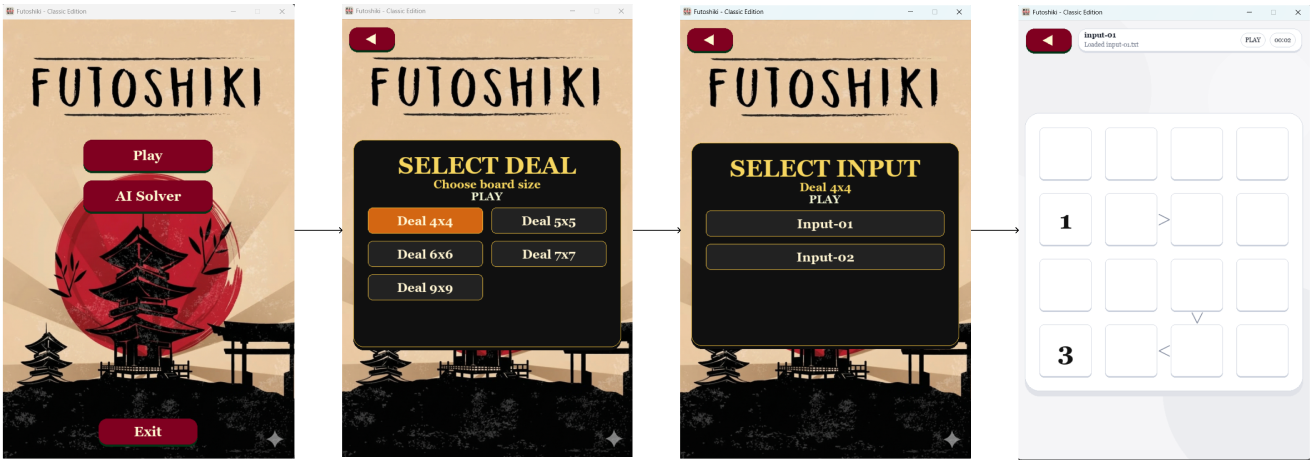
\includegraphics[width=0.9\linewidth]{image/gui_screen.png}
    \caption{GUI screen flow from menu to gameplay.}
    \label{fig:gui-screen-flow}
\end{figure}

\subsubsection{Gameplay Interface}
The gameplay screen renders the grid, keeps clue cells fixed, and validates moves in real time. Main controls:
\begin{itemize}
    \item click to select a cell;
    \item keys \(1\) to \(N\) to fill values;
    \item Backspace/Delete/0 to clear;
    \item timer display.
\end{itemize}
Inequality symbols are shown between cells, and completion is announced when all constraints are satisfied.

\begin{figure}[H]
    \centering
    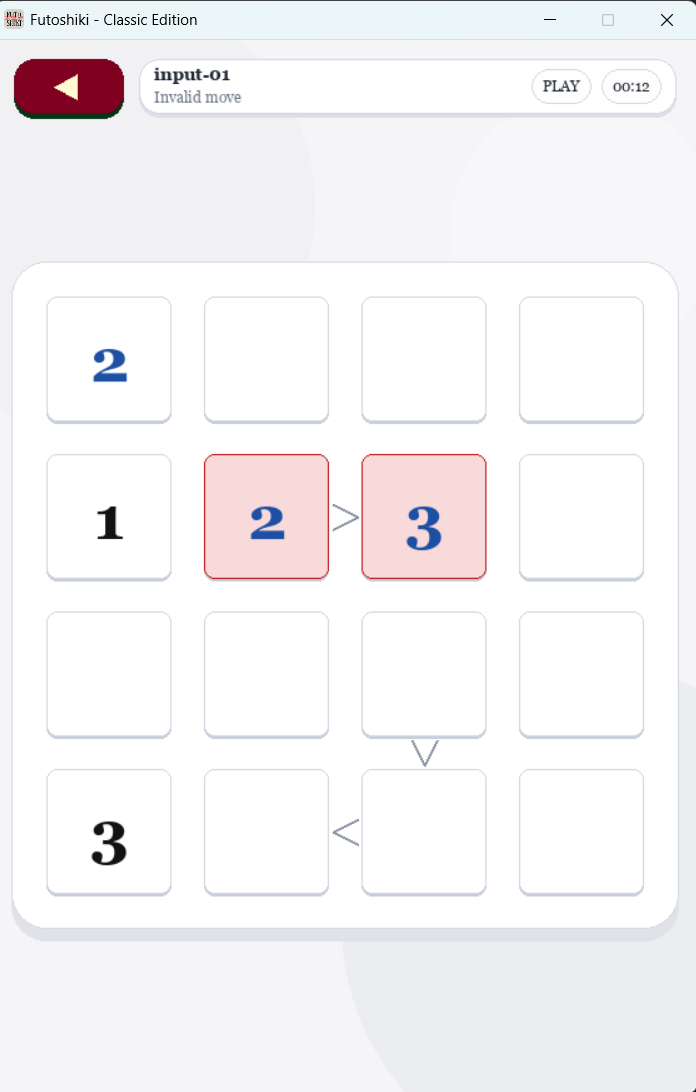
\includegraphics[width=0.9\linewidth]{image/gameplay.png}
    \caption{Main gameplay interface in manual mode.}
    \label{fig:gui-gameplay}
\end{figure}

\subsubsection{AI Solver Visualization}
AI visualization is handled by \texttt{AISolverManager} with a worker thread and step queue, so the UI remains responsive while solving. Solver steps are streamed incrementally to the board so users can observe the solving process.

Key behaviors:
\begin{itemize}
    \item highlight current solver actions;
    \item distinguish backtracking steps;
    \item allow skipping remaining animation;
    \item validate final state before showing solved status.
\end{itemize}

\begin{figure}[H]
    \centering
    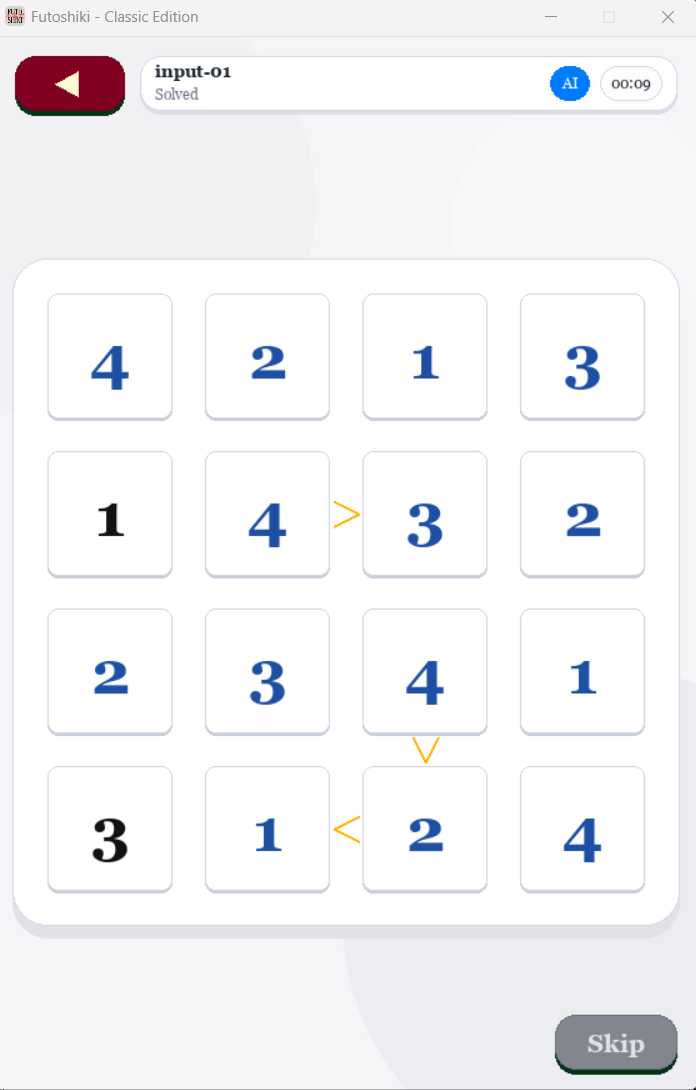
\includegraphics[width=0.9\linewidth]{image/ai_solver.png}
    \caption{Step-by-step AI solver visualization on the game screen.}
    \label{fig:gui-ai-animation}
\end{figure}

\subsubsection{Visual Design}
The visual style is simple and consistent to prioritize board readability and solver progress. Reusable UI components keep interactions uniform and implementation complexity low.

Overall, the GUI bridges puzzle data, user interaction, and solver execution in a practical way.

\section{Experimental Evaluation}
This section presents a comprehensive evaluation of four search algorithms: Breadth-First Search (BFS), Depth-First Search (DFS), Uniform Cost Search (UCS), and $A^*$ applied to the FreeCell card game solver.

\subsection{Experimental Setup}
To ensure a fair comparison, all algorithms were tested under the following conditions:
\begin{itemize}
    \item \textbf{Performance Metrics:} Assessment was based on peak memory usage, expanded nodes, runtime, solution step quality, and success rate.
    \item \textbf{Resource Constraints:} A maximum of 500,000 nodes and a 30-second timeout per game instance.
    \item \textbf{Test Data:} 10 benchmark cases (\texttt{game\_00} through \texttt{game\_09}) executed under identical hardware conditions.
\end{itemize}

\subsection{Performance Summary}
The empirical data shows that \textbf{$A^*$} delivers the best overall performance, particularly in runtime and success rate.
\begin{figure}[H] % [H] sẽ giữ ảnh đúng vị trí này
    \centering
    \includegraphics[width=0.9\textwidth]{image/overview_table.png}
    \caption{Summary of average performance across all metrics. Green = best, Red = worst}
    \label{fig:performance_chart}
\end{figure}

\subsection{Metric 01 --- Peak Memory Usage}
\label{metric-01-peak-memory-usage}

\begin{figure}[H]
    \centering
    \includegraphics[width=0.85\textwidth]{image/average_peak_memory_usage.png}
    \caption{Average Peak Memory Usage by Algorithm (10 Test Cases) }
    \label{fig:memory_usage}
\end{figure}

\subsubsection{Analysis}
\label{analysis}

\begin{description}
    \item[DFS (84.5 MB) --- Best:] 
    The Iterative Deepening Search (IDS) implementation in \texttt{dfs.py} uses an explicit recursion stack that only holds the current path to the active node, plus a visited dictionary scoped to the current depth iteration. Crucially, this dictionary is discarded and rebuilt at each new depth limit, meaning DFS never accumulates a large persistent frontier. The memory footprint grows roughly linearly with the depth limit, not exponentially with the branching factor.

    \item[A* (142.7 MB) --- Second Best:] 
    $A^*$ in \texttt{a\_star.py} maintains a heap-based frontier and a \texttt{best\_cost} dictionary. The heuristic functions (\texttt{heuristic\_blocking} and \texttt{heuristic\_foundation\_gap}) actively guide the search toward productive states, meaning fewer states are ever added to the heap. The blocking heuristic specifically penalizes states with many cards blocking foundation targets, causing the algorithm to prune entire subtrees before they enter memory.

    \item[BFS (209.8 MB) --- High:]  
    BFS in \texttt{bfs.py} maintains a reached set containing every state ever enqueued --- a strict BFS graph-search rule that prevents re-expansion but requires storing the full exploration frontier. Since FreeCell has a very high branching factor, this set grows rapidly. The \texttt{deque} queue itself also holds full state objects, contributing significantly to the memory total.

    \item[UCS (228.6 MB) --- Worst:]  
    UCS in \texttt{ucs.py} maintains both a \texttt{heapq} priority queue and a \texttt{best\_g} dictionary mapping visited states to their lowest costs. Because UCS re-expands states when a cheaper path is found, more entries accumulate in \texttt{best\_g} compared to BFS's simple seen-once reached set. The combination of priority queue overhead and the dynamic cost structure means UCS retains the most state objects in memory simultaneously.
\end{description}

\subsubsection{Key Takeaway}
\label{key-takeaway}

\textbf{Conclusion on Resource Efficiency:} 
DFS is the only algorithm suitable for highly memory-constrained environments. $A^*$ offers a practical middle ground. In contrast, BFS and UCS are unsuitable when RAM is a bottleneck, as their memory usage scales with the size of the explored state space rather than the solution depth.

\subsection{Metric 02 --- Average Expanded Nodes}
\label{metric-02-average-expanded-nodes}

\begin{figure}[H]
    \centering
    \includegraphics[width=0.85\textwidth]{image/average_expanded_nodes.png}
    \caption{Average Expanded Nodes by Algorithm (10 Test Cases)}
    \label{fig:expanded_nodes}
\end{figure}

\subsubsection{Analysis}
\label{analysis-1}

\begin{description}
    \item[$A^*$ (22,542) --- Best:] 
    $A^*$ achieves the lowest expansion count by combining actual cost ($g$) with heuristic estimate ($h$). The \texttt{heuristic\_blocking} function counts cards physically blocking the next card needed for foundation piles, providing a tight lower bound that allows $A^*$ to reject large portions of the state space. This demonstrates the core value of informed search, where the algorithm focuses computation only on promising directions.

    \item[UCS (49,317) --- Second Best:] 
    UCS benefits from the asymmetric cost function defined in \texttt{get\_move\_cost()} within \texttt{ucs.py}. By assigning foundation moves a cost of 1 unit and free cell moves 50 units, the algorithm receives implicit guidance to reward progress. As a result, UCS expands significantly fewer states than BFS despite using similar graph-search guarantees.

    \item[BFS (94,900) --- High:] 
    BFS expands states in strict order of depth. It treats all moves as equal one-step transitions, making no distinction between a move to foundation and parking in a free cell. Consequently, BFS wastes substantial effort exploring shallow, unproductive states before reaching productive branches of the search tree.

    \item[DFS (156,602) --- Worst:] 
    The high expansion count is a direct result of the IDS implementation, which must repeat entire DLS iterations for each new depth limit. Because FreeCell solutions rarely exist at shallow depths, DFS iterates through many fruitless limits, repeatedly expanding the same early states and inflating the total count relative to the actual solution depth.
\end{description}

\subsubsection{Key Takeaway}
\label{key-takeaway-1}

\textbf{Impact of Informed Search:}
The nearly 7x difference between $A^*$ (22,542) and DFS (156,602) demonstrates that heuristic design quality is the most critical factor in determining expansion efficiency.
\subsection{Metric 03 --- Average Runtime}\label{metric-03-average-runtime}
\begin{figure}[H] % [H] sẽ giữ ảnh đúng vị trí này
    \centering
    \includegraphics[width=0.9\textwidth]{image/average_runtime.png}
    \caption{Average Runtime by Algorithm (10 Test Cases)}
    \label{fig:performance_chart}
\end{figure}
\subsubsection{Analysis}\label{analysis-2}




\begin{description}
    \item[$A^*$ (30.15 s) --- Best:] 
    $A^*$'s runtime advantage directly mirrors its node efficiency. By expanding only 22,542 nodes on average, the algorithm performs significantly fewer heap operations ($O(\log n)$), state hash computations, and successor generations. Additionally, the move priority ordering in \texttt{\_move\_priority()} reduces wasted evaluations, making $A^*$ approximately 4.6x faster than DFS and 2.6x faster than BFS.

    \item[UCS (80.06 s) --- Second Best:] 
    Despite having fewer expansions than BFS, UCS is not drastically faster due to the overhead of priority queue maintenance. Each expansion requires comparing complex tuples and performing \texttt{heapq} operations, which are more computationally expensive than BFS's $O(1)$ operations. However, cost-guided pruning still yields a roughly 8\% speed improvement over BFS.

    \item[BFS (87.46 s) --- Third:] 
    BFS remains competitive because its \texttt{deque} operations are $O(1)$ compared to the $O(\log n)$ overhead of a heap. This simpler data structure partially compensates for the higher node expansion count. BFS also benefits from "short-circuiting" by checking \texttt{is\_goal()} immediately when a successor is generated.

    \item[DFS (137.60 s) --- Worst:] 
    DFS suffers from the massive redundancy of IDS re-execution. For a solution at depth 60, DFS executes 59 failed search passes before the successful one, making the total runtime proportional to the sum of work across all depth iterations. Furthermore, the recursive \texttt{\_dls()} function incurs Python call stack overhead, adding significant latency.
\end{description}

\subsubsection{Key Takeaway}
\label{key-takeaway-2}

\textbf{Computational Efficiency:}
Runtime correlates strongly with node expansions but is heavily influenced by data structure overhead. $A^*$ is the only algorithm capable of operating within a tight real-time budget, as the others frequently approach or exceed the 30-second timeout in complex game instances.

\subsection{Metric 04 --- Average Solution Steps}
\label{metric-04-average-solution-steps}

\begin{figure}[H]
    \centering
    \includegraphics[width=0.85\textwidth]{image/average_solution_steps.png}
    \caption{Average Solution Steps by Algorithm (10 Test Cases)}
    \label{fig:solution_steps_chart}
\end{figure}

\subsubsection{Analysis}
\label{analysis-3}

\begin{description}
    \item[BFS (59.8 steps) --- Best:] 
    BFS is theoretically guaranteed to return the shortest path for unit-cost problems because it explores all states at depth $d$ before any state at $d+1$. Since it treats every move as equal, the first time it reaches a goal, it has arrived via the minimum number of steps. The 59.8 average represents the true optimal step count for this test set.

    \item[DFS (60.5 steps) --- Near-Optimal:] 
    The IDS implementation produces solutions nearly as short as BFS because it finds a solution at the smallest depth limit where one exists. The minor gap of 0.7 steps occurs because IDS uses a path-based visited check rather than a global one, occasionally allowing for slightly suboptimal paths at the same depth level.

    \item[UCS (69.8 steps) --- Cost-Optimal:] 
    UCS is designed to minimize total accumulated cost rather than the number of steps. Due to asymmetric weights in \texttt{get\_move\_cost()} (foundation moves cost 1 while free cell moves cost 50), UCS may prefer a longer path that avoids expensive free cell parking. The 69.8 average reflects this trade-off between total cost and total steps.

    \item[$A^*$ (90.0 steps) --- Longest:] 
    $A^*$ produces the longest solutions because it optimizes for the combined cost $f = g + h$ using the same asymmetric weights as UCS. The \texttt{heuristic\_blocking} function reinforces this by penalizing states that block foundations. This often leads $A^*$ through "cleaner" but physically longer routes to minimize the overall game cost.
\end{description}

\subsubsection{Key Takeaway}
\label{key-takeaway-3}

\textbf{Path Quality vs. Cost Efficiency:}
While BFS and DFS (IDS) provide the shortest paths, UCS and $A^*$ prioritize cost efficiency. If minimizing the raw number of moves is the priority, BFS is the ideal choice. However, for applications where avoiding board congestion (free cell usage) is more critical, $A^*$ and UCS produce structurally superior solutions despite their length.

\subsection{Metric 05 --- Success Rate}
\label{metric-05-success-rate}

\begin{figure}[H]
    \centering
    \includegraphics[width=0.85\textwidth]{image/success_rate.png}
    \caption{Success Rate by Algorithm (10 Test Cases)}
    \label{fig:success_rate_chart}
\end{figure}

\subsubsection{Analysis}
\label{analysis-4}

\begin{description}
    \item[$A^*$ (90\%) --- Best:] 
    $A^*$ successfully solves 9 out of 10 games because its heuristic dramatically reduces the effective search space. Even on harder instances where BFS and UCS exhaust the 500,000-node budget, $A^*$'s guided expansion finds solutions using far fewer resources. The 10\% failure rate likely occurs in "heavily locked" board configurations where foundation targets are deeply buried, providing insufficient guidance for the heuristic.

    \item[DFS (50\%) --- Second:] 
    DFS benefits from a low memory footprint, avoiding the out-of-memory issues that affect BFS and UCS. However, the overhead of IDS re-execution often causes DFS to hit the 30-second time limit, especially in games requiring more than 80 moves. Its success rate reflects a direct balance between its memory advantage and its time disadvantage.

    \item[UCS (50\%) --- Second (Tied):] 
    UCS shares the same success rate as DFS but fails due to node exhaustion rather than time. Its broad expansion pattern and 228.6 MB memory usage often fill the priority queue and hit the 500,000-node limit before finding a solution. While cost-guided search provides an advantage over plain BFS, the lack of a true heuristic remains a bottleneck for complex boards.

    \item[BFS (40\%) --- Worst:] 
    Despite being theoretically complete, BFS is the most wasteful algorithm under real-world constraints. It expands states blindly in breadth order without prioritizing promising paths, causing it to reach binding node and time limits prematurely. BFS succeeds only on simpler instances where the solution is reachable within the narrow constraint window.
\end{description}

\subsubsection{Key Takeaway}
\label{key-takeaway-4}

\textbf{Practical Necessity of Heuristics:}
Under strict resource constraints, success rate is the ultimate performance metric. The 50-percentage-point gap between $A^*$ and BFS demonstrates that heuristic search is not merely an optimization but a practical necessity for solving FreeCell games of non-trivial difficulty.

\subsection{Overview --- Holistic Comparison}
\label{overview-holistic-comparison}

\begin{figure}[H]
    \centering
    \includegraphics[width=0.85\textwidth]{image/overview_radar.png}
    \caption{Overview Performance Radar Across 10 Test Cases}
    \label{fig:holistic_radar}
\end{figure}

\subsubsection{Cross-Metric Insights}
\label{cross-metric-insights}

\begin{description}
    \item[1. The Memory-Speed Paradox in DFS:] 
    DFS exhibits a highly counterintuitive profile by utilizing the least memory (84.5 MB) while being the slowest algorithm (137.60s) and expanding the most nodes (156,602). This occurs because the IDS mechanism saves memory by discarding previously computed work, requiring 60--90 complete search passes to find a solution at those depths.

    \item[2. The $A^*$ Step-Count Paradox:] 
    Despite being the fastest and most resource-efficient, $A^*$ produces the longest average solutions at 90.0 steps. This is a direct consequence of optimizing a non-uniform cost function where foundation moves (cost 1) are heavily favored over free cell moves (cost 50), leading to longer but more cost-efficient routes.

    \item[3. Success Rate as the Binding Constraint:] 
    Under limited resources, success rate becomes the dominant metric. $A^*$'s ability to solve 90\% of games within 30 seconds proves that for production deployment, a well-tuned heuristic search is a practical necessity rather than a mere optimization.

    \item[4. UCS vs. BFS Trade-off:] 
    UCS expands nearly 50\% fewer nodes than BFS, yet only yields a modest 8\% runtime improvement. This demonstrates that the priority queue overhead partially negates the benefits of fewer expansions, supporting the case that a true heuristic ($A^*$) is required for substantial performance gains.
\end{description}
\section{Conclusion}
This project delivers a complete Futoshiki-solving system that combines multiple AI paradigms with an interactive GUI. Experiments confirm clear trade-offs among search, logic inference, and SAT in runtime, memory, and node expansion.

The codebase is organized for reproducibility and extension, with standardized I/O, solver abstractions, and automated tests. The implementation stack remains lightweight and aligned with requirements (\texttt{pygame}, \texttt{python-sat}, \texttt{pytest}).

Overall, the objectives were achieved: correct constraint modeling, implementation of representative methods, benchmark-based evaluation, and clear presentation through both CLI and GUI workflows.
\section{References}
[Chèn nội dung tại đây]
\appendix
\section{Appendix}
\subsection{Generative AI Usage Disclosure}
This section documents the use of Large Language Models (LLMs) during the development of this project:
\begin{itemize}
	\item \textbf{AI Tools Used}: Gemini, ChatGPT, Claude.
	\item \textbf{Usage Scenarios}:
	\begin{itemize}
		\item Code debugging and optimization for search algorithms.
		\item Formatting the LaTeX report and troubleshooting matplotlib diagrams.
		\item Refining English grammar in the documentation.
	\end{itemize}
	\item \textbf{Sample Prompts}:
	\begin{itemize}
		\item ``How should I enforce row/column uniqueness and inequality constraints efficiently in a Futoshiki backtracking solver?''
		\item ``In our A* Futoshiki solver, what is a good admissible heuristic to reduce node expansions on 7x7 and 9x9 inputs?''
		\item ``Help me format a LaTeX table that compares runtime, memory, and expanded nodes across Backtracking, Forward Chaining, Backward Chaining, SAT, and A* for the 10 input files.''
	\end{itemize}
\end{itemize}

\subsection{Project Deliverables}
\begin{itemize}
	\item \textbf{Demo Video}: A video demonstrating the GUI, manual gameplay, and solver animations can be found at: Click to see video.
	\item \textbf{Futoshiki-Puzzles Project Repository, GitHub}: \href{https://github.com/Chistaif/Futoshiki-Puzzles}{Click to see repository}
\end{itemize}

\subsection{Additional Tables and Charts}
[Chèn nội dung tại đây]

\end{document}
